 \documentclass[conference]{IEEEtran}

%Template version as of 6/27/2024

\usepackage{cite}
\usepackage{amsmath,amssymb,amsfonts}
\usepackage{algorithmic}
\usepackage{graphicx}
\usepackage{textcomp}
\usepackage{xcolor}
\def\BibTeX{{\rm B\kern-.05em{\sc i\kern-.025em b}\kern-.08em
    T\kern-.1667em\lower.7ex\hbox{E}\kern-.125emX}}
\begin{document}

\title{LiTerm: An Independent File Editor, Assembler, and Processor}

\author{

\IEEEauthorblockN{Tsegazeab Beteselassie}
\IEEEauthorblockA{\textit{Department of EECS} \\
\textit{Massachusetts Institute of Technology}\\
Cambridge, MA \\
tsegaz@mit.edu}

\and

\IEEEauthorblockN{Ziyad Hassan}
\IEEEauthorblockA{\textit{Department of EECS} \\
\textit{Massachusetts Institute of Technology}\\
Cambridge, MA \\
zhassan3@mit.edu}

\and

\IEEEauthorblockN{Simon Opsahl}
\IEEEauthorblockA{\textit{Department of EECS} \\
\textit{Massachusetts Institute of Technology}\\
Cambridge, MA \\
sopsahl@mit.edu}
}

\maketitle

\begin{abstract}
  We present a design for a terminal-based text editor fully supported in hardware on a Xilinx FPGA. We utilize a independent RISC-V processor that runs assembler code located in instruction memory. Separate from the processor exists a terminal-based text editor that accepts PS2 keyboard input and allows for dynamic program file editing. We propose a system that performs the reduction of assembly code to binaries entirely on the FPGA. Performance and output are measured through a debugger communicating over UART and a separate MMO visualization of data memory.
\end{abstract}

\begin{IEEEkeywords}
digital design, field programmable gate array, assembly, processor, terminal
\end{IEEEkeywords}

\section{Physical System}
Our design consists of four physical components:
\begin{itemize}
    \item FPGA: We use a Real Digital Urbana FPGA development board provided by the course staff of 6.205: Digital Systems Laboratory. Most of the text editor, assembler, processor, and visualization components are hosted here.
    \item Monitor: We connect to a 720p monitor by HDMI. The monitor visualizes the terminal display, text editor, and MMO plotting.
    \item Keyboard: We use a PS2 keyboard connected to the FPGA by cable and a MDFLY breakout board. The keyboard is used for generating assembly code and branching to different parts of the program.
    \item Host: We run a debugger program communicating over UART in Python on a host computer. This is used for program verification, visualization, and additional program features.
\end{itemize}


\begin{figure}
    \centering
    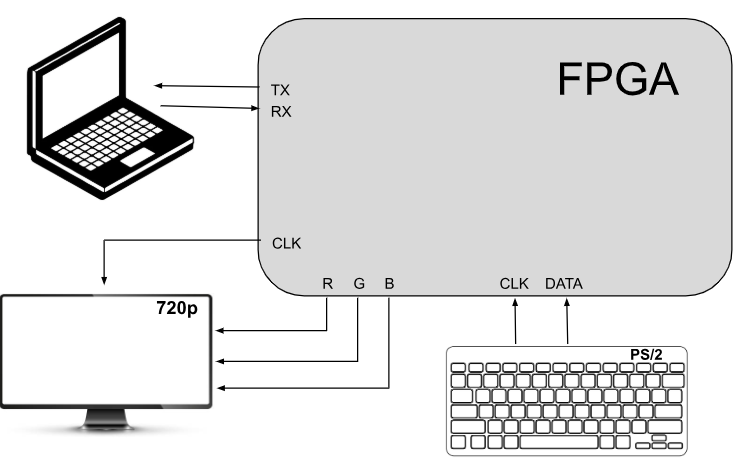
\includegraphics[width=1\linewidth]{physical_system.png}
    \caption{Overall Physical System}
    \label{fig:enter-label}
\end{figure}



\subsection{Monitor}
% Talk about communication, frame buffer, and NOT character sprite stuff. That'll go later. Just frame buffer to comm...
Any inputs sent to the terminal controller are used to display characters onto the 720p HDMI monitor. Based on the input received, the terminal controller will send the appropriate signal to the character sprite module, which is what draws the correct character on the screen. In addition to this, a buffer module will be keeping track of the full line being typed onto the terminal. Once the enter key is pressed, the full terminal line will be sent to the processor to run the relevant instruction.

\begin{figure}
    \centering
    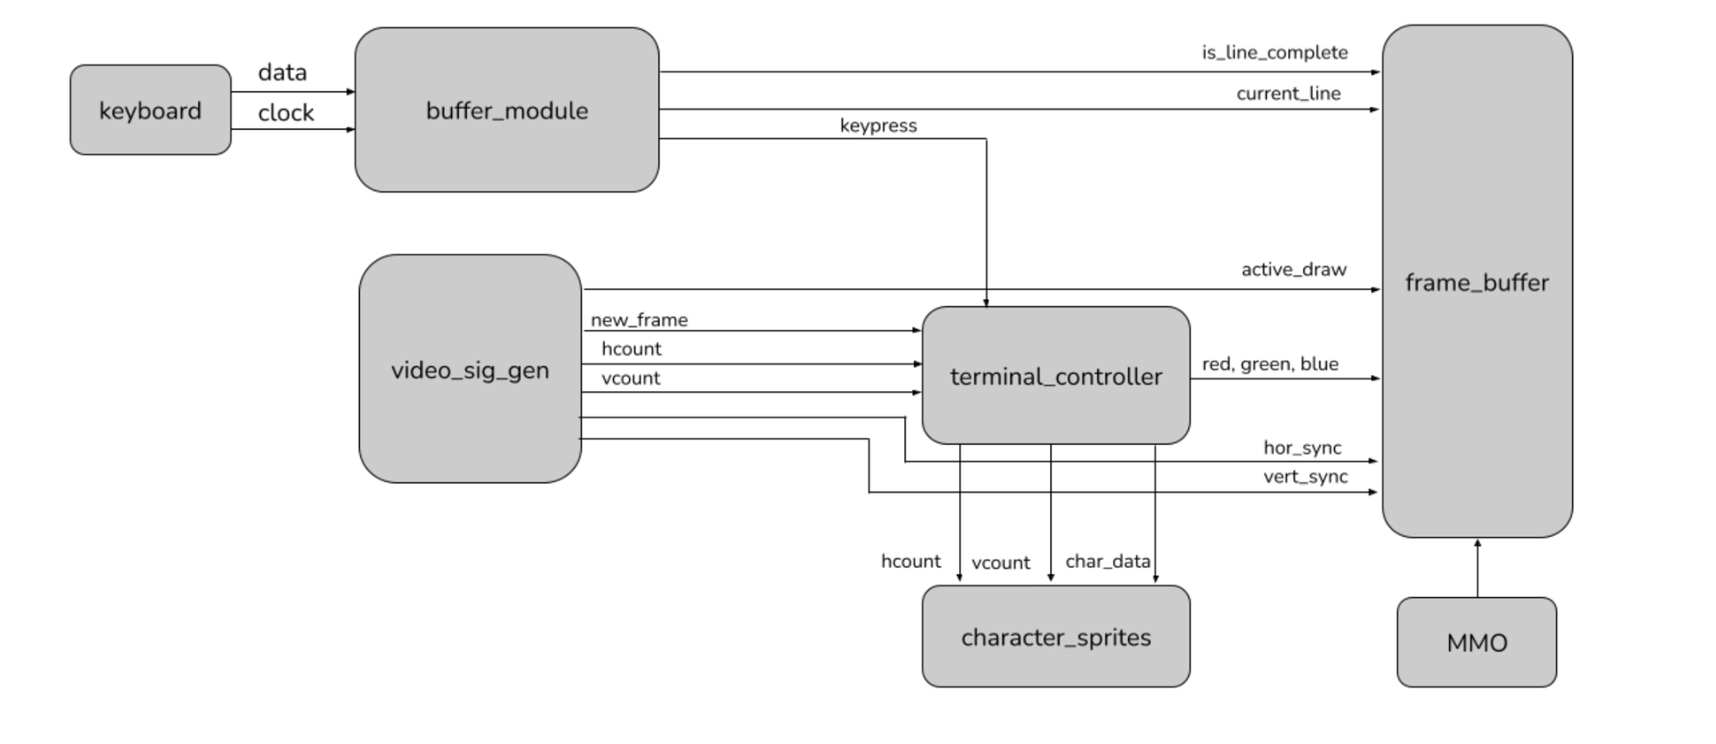
\includegraphics[width=1\linewidth]{terminal_conroller.png}
    \caption{Terminal and Display Block Diagram}
    \label{fig:enter-label}
\end{figure}

\subsection{Keyboard}
% Talk about communication, hardware, and decoder. That's all...
The main pieces of external hardware for LiTerm are the PS2 keyboard and the 720p HDMI monitor. For device-to-host communication, the PS2 keyboard sends data as follows: 1 start bit, 8 data bits (LSB first), 1 parity bit, and 1 stop bit. This data is sent into the buffer module, which will decode the keyboard inputs and send them to the terminal controller, as well as store the current line being typed. Characters will be displayed onto the monitor using the TMDS protocol used in the HDMI protocol. The relevant hcount, vcount, and active signals will be generated for a 720p monitor.


\subsection{Host}
% Talk about python debugger and uart connection. Breifly talk about protocols 
The host is used to run debugging protocols concurrently. When we are in debugger mode, the debugger has access to reading/writing in data memory, program memory, and in the program file. At the very least, this allows for verification of each individual piece of the system. It also permits profiling of results and visualizing state dumps. When a program is executed in debugger mode, we can visualize on the host how the register values and data memory evolve over the course of the program execution. 

The host communicates with the device over UART, and it requires certain protocols to initiate where it is accessing memory, how much it means to access, and whether or not we expect a read or a write. This protocol is the first byte sent by the host that leads to the sending of data either by the host to load memory or by the device to profile it. The device is only listening when in debugger mode. The breakdown of the protocol is enumerated in Figure 3.

The location determines what memory we access (text editor buffer, progmem, datamem, and processor registers). The width determines what the size of the data we read is (32 bit for all but text editor buffer). The depth is the amount of data we read or write, corresponding to a 4 bit value representing 16 different sizes to dump or load for each memory location. This also is used to generate the time that both the host and device wait in sending the signal before proceeding to other tasks.


\begin{figure}
    \centering
    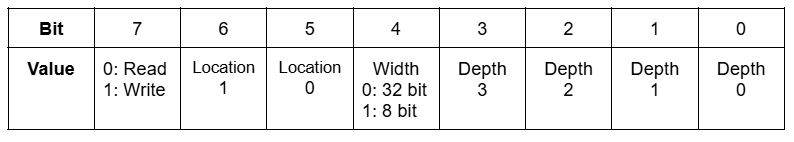
\includegraphics[width=1\linewidth]{protocol.png}
    \caption{Host-Device Communication Protocol}
    \label{fig:enter-label}
\end{figure}


\section{Control Flow}
% Talk about branching and the commands for a certain input (debugger triggers, commands)
To control our program flow and simplify our process we use our FPGA buttons and switches to indicate what part of the process we want to execute

\begin{itemize}
    \item Button 2: brings up the text editor
    \item Button 3: Compiles the text on the text editor to binary 
    \item Button 4: If error free program, run processor on program 
    \item Switch 0: Debugger mode on/off
    \item Switch 1: Visualization mode on/off
\end{itemize}
\subsection{Terminal Display}
The status of the processor will be displayed on the terminal, on the bottom row of the screen. The possible states of the terminal are as follows: "processor idle", "processor running", "compilation succeeded", "compilation failed", and "visualizing".
\newline\newline
By default, the processor is idle, and the monitor will display the current command being written, as well as any previous commands, in a terminal-like format. If button 2 is pressed, the text editor gets brought up, clearing the monitor screen and allowing the user to type what they'd like.
\newline\newline
If button 3 is pressed, anything written in the text editor gets compiled and the result of that is displayed as either success or failure on the terminal. If the compilation is successful and the program is executed, the state is now "compilation succeeded". Otherwise, it becomes "compilation failed".
\newline\newline
If the program is executed with the visualizer enabled, then the MMO will be displayed and the speed of execution will be slowed to show how the states of the register change. The MMO will be a bar graph, where each grid square on the x-axis represents a register, and the height of the graph at that location representing its value. For a program such as bubblesort, at each step of execution, the heights of the different registers will change, showing how the registers go from sorted to unsorted. The state will also transition to "visualizing."
\subsection{Text Editor}
% Talk about sprite logic, the storage of the page, the code editor, etc
% ...


Both the character sprites and the current state of the terminal are stored using BRAM modules. The character sprites were turned into a spritesheet and palletized, with the relevant portion of the spritesheet being cut out and displayed for each part of the terminal. The terminal display itself is split up into a grid, with each grid square containing a number corresponding to the character it contains. The grid values are stored in a BRAM and updated with every keypress.
Within the text editor, we dynamically edit the program file, which stores the 256 potential lines of code.

\subsection{Assembler}
When we assemble the code in the text editor, we rely on several design choices:
\begin{itemize}
    \item All registers must be in the format `x\_\_'.
    \item All immediate values must be hexadecimal and preceded by `h'. 
    \item All text after `\#' in a line will be ignored.
    \item Labels must be in the format `:LABEL:', and the length of the label must be no longer than 8 characters. When used in a branching instruction, the colons must also be included (`j :LABEL:').
\end{itemize}
These design choices ensure that the assembly step proceeds consistently, and it limits the amount of syntax difference that need be supported. If all these design choices are followed, and the instruction syntax obeys what is to be expected, then the assembler should work. If they are not obeyed, then the terminal will display the error and the line it corresponds to (i.e. `Syntax error on line \_\_\_.'). 

The process of assembling the code requires several distinct steps:
\begin{enumerate}
    \item We have a 256 bit map that corresponds to whether or not a line is to be considered. All bits are initialized to 0. Iterate through each line. If the first character that is not a space or tab is not `\#' or `:' and the line is not empty, set that line's value to 1.
    \item We have a buffer that maps up to 8 labels to corresponding 8 bit program counters. Iterate through the lines again. If the first character (that is not space or tab) is a `:', add the enclosed label to the buffer with the corresponding PC (sum of all of the preceding bits in the map plus 1). 
    \item Now go line by line through the lines with a mapping of 1:
    \begin{enumerate}
        \item Get the instruction as the first string separated by space, tab, and comma delimiters. Determine what to expect next (i.e. reg, reg, imm). 
        \item For the remaining strings, decode the item and add it into the instruction encoding. 
        \item Return the opcode if no syntax errors have been encountered.
    \end{enumerate}
    The returned opcode is added to the program memory at the corresponding PC.
\end{enumerate}

As stated before, the assembler will break if any syntax is violated and return the line that the error was first encountered. 


\subsection{Processor}
\begin{figure}
    \centering
    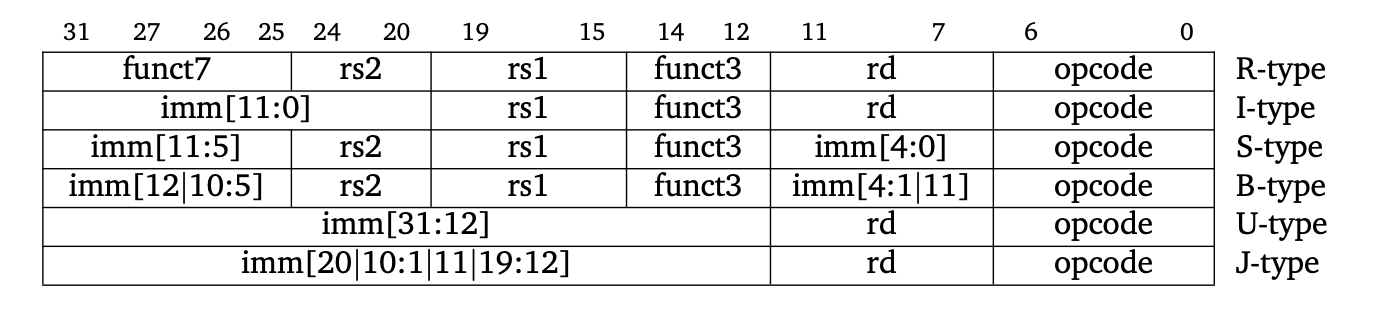
\includegraphics[width=1\linewidth]{Riscv instruction type .png}
    \caption{32 bit instruction template}
    \label{fig:enter-label}
\end{figure}

For our processor we'll be using a standard 4 stage pipeline Risc-V processor. The ISA that we use for this will be a Risc-v Base Integer 32I instruction set without ebreak and ecall, since we won't be using an OS. This ISA will be shared with the assembler so that when the assembler receives instructions, it'll translate it to 32 bit instructions that the processor understands. The processor will grab the instructions from a BRAM that is initialized from a ".mem" file that the assembler writes to. The processor will be using a data-shared memory, so other processes can also access values written to by the processor. We don't need any concurrency controls since the other processes(visualization and debugging) are read-only. In accordance with the MMO agreement, the first 720 spots in data memory will only be touched by the processor if it's part of the MMO any other data operation will be offset by 720. 


\section{Visualization}
We have few updates in this area, but the plan is to take the first 720 values in data memory and map them through MMO to a separate frame buffer displaying each value's magnitude as the length of the corresponding line. As the lines are sorting we'll use a PWM module to hear the "progress" of the program sorting. To enable this application we plan to slow the processor down by down cycling its clock and show the results of a sorting algorithm on the elements of a list so that the human eye can catch it and the sound doesn't go too fast
An example visualization is shown in Figure 5. 
\begin{figure}
    \centering
    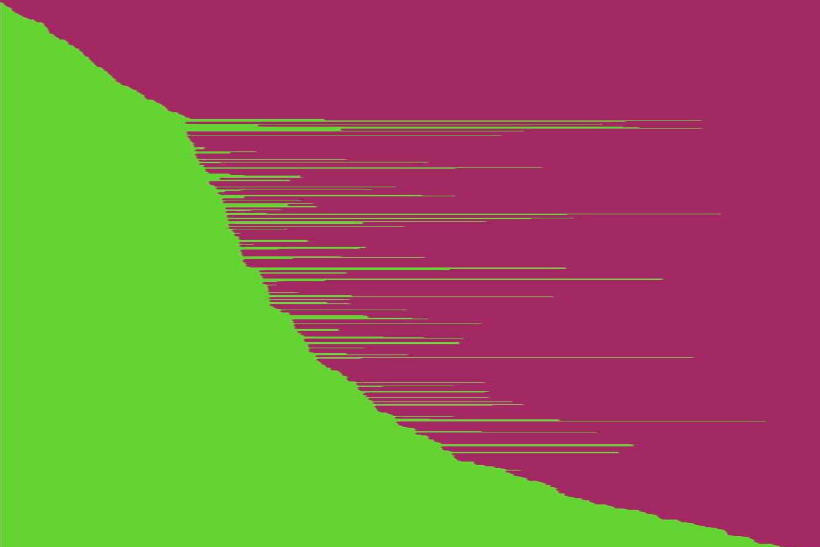
\includegraphics[width=1\linewidth]{MMO.png}
    \caption{Data Memory Mapped Visualization}
    \label{fig:enter-label}
\end{figure}


\end{document}